% Options for packages loaded elsewhere
\PassOptionsToPackage{unicode}{hyperref}
\PassOptionsToPackage{hyphens}{url}
\PassOptionsToPackage{dvipsnames,svgnames,x11names}{xcolor}
%
\documentclass[
  letterpaper,
  DIV=11,
  numbers=noendperiod]{scrartcl}

\usepackage{amsmath,amssymb}
\usepackage{iftex}
\ifPDFTeX
  \usepackage[T1]{fontenc}
  \usepackage[utf8]{inputenc}
  \usepackage{textcomp} % provide euro and other symbols
\else % if luatex or xetex
  \usepackage{unicode-math}
  \defaultfontfeatures{Scale=MatchLowercase}
  \defaultfontfeatures[\rmfamily]{Ligatures=TeX,Scale=1}
\fi
\usepackage{lmodern}
\ifPDFTeX\else  
    % xetex/luatex font selection
\fi
% Use upquote if available, for straight quotes in verbatim environments
\IfFileExists{upquote.sty}{\usepackage{upquote}}{}
\IfFileExists{microtype.sty}{% use microtype if available
  \usepackage[]{microtype}
  \UseMicrotypeSet[protrusion]{basicmath} % disable protrusion for tt fonts
}{}
\makeatletter
\@ifundefined{KOMAClassName}{% if non-KOMA class
  \IfFileExists{parskip.sty}{%
    \usepackage{parskip}
  }{% else
    \setlength{\parindent}{0pt}
    \setlength{\parskip}{6pt plus 2pt minus 1pt}}
}{% if KOMA class
  \KOMAoptions{parskip=half}}
\makeatother
\usepackage{xcolor}
\setlength{\emergencystretch}{3em} % prevent overfull lines
\setcounter{secnumdepth}{5}
% Make \paragraph and \subparagraph free-standing
\ifx\paragraph\undefined\else
  \let\oldparagraph\paragraph
  \renewcommand{\paragraph}[1]{\oldparagraph{#1}\mbox{}}
\fi
\ifx\subparagraph\undefined\else
  \let\oldsubparagraph\subparagraph
  \renewcommand{\subparagraph}[1]{\oldsubparagraph{#1}\mbox{}}
\fi


\providecommand{\tightlist}{%
  \setlength{\itemsep}{0pt}\setlength{\parskip}{0pt}}\usepackage{longtable,booktabs,array}
\usepackage{calc} % for calculating minipage widths
% Correct order of tables after \paragraph or \subparagraph
\usepackage{etoolbox}
\makeatletter
\patchcmd\longtable{\par}{\if@noskipsec\mbox{}\fi\par}{}{}
\makeatother
% Allow footnotes in longtable head/foot
\IfFileExists{footnotehyper.sty}{\usepackage{footnotehyper}}{\usepackage{footnote}}
\makesavenoteenv{longtable}
\usepackage{graphicx}
\makeatletter
\def\maxwidth{\ifdim\Gin@nat@width>\linewidth\linewidth\else\Gin@nat@width\fi}
\def\maxheight{\ifdim\Gin@nat@height>\textheight\textheight\else\Gin@nat@height\fi}
\makeatother
% Scale images if necessary, so that they will not overflow the page
% margins by default, and it is still possible to overwrite the defaults
% using explicit options in \includegraphics[width, height, ...]{}
\setkeys{Gin}{width=\maxwidth,height=\maxheight,keepaspectratio}
% Set default figure placement to htbp
\makeatletter
\def\fps@figure{htbp}
\makeatother

\KOMAoption{captions}{tableheading}
\makeatletter
\makeatother
\makeatletter
\makeatother
\makeatletter
\@ifpackageloaded{caption}{}{\usepackage{caption}}
\AtBeginDocument{%
\ifdefined\contentsname
  \renewcommand*\contentsname{Table of contents}
\else
  \newcommand\contentsname{Table of contents}
\fi
\ifdefined\listfigurename
  \renewcommand*\listfigurename{List of Figures}
\else
  \newcommand\listfigurename{List of Figures}
\fi
\ifdefined\listtablename
  \renewcommand*\listtablename{List of Tables}
\else
  \newcommand\listtablename{List of Tables}
\fi
\ifdefined\figurename
  \renewcommand*\figurename{Figure}
\else
  \newcommand\figurename{Figure}
\fi
\ifdefined\tablename
  \renewcommand*\tablename{Table}
\else
  \newcommand\tablename{Table}
\fi
}
\@ifpackageloaded{float}{}{\usepackage{float}}
\floatstyle{ruled}
\@ifundefined{c@chapter}{\newfloat{codelisting}{h}{lop}}{\newfloat{codelisting}{h}{lop}[chapter]}
\floatname{codelisting}{Listing}
\newcommand*\listoflistings{\listof{codelisting}{List of Listings}}
\makeatother
\makeatletter
\@ifpackageloaded{caption}{}{\usepackage{caption}}
\@ifpackageloaded{subcaption}{}{\usepackage{subcaption}}
\makeatother
\makeatletter
\@ifpackageloaded{tcolorbox}{}{\usepackage[skins,breakable]{tcolorbox}}
\makeatother
\makeatletter
\@ifundefined{shadecolor}{\definecolor{shadecolor}{rgb}{.97, .97, .97}}
\makeatother
\makeatletter
\makeatother
\makeatletter
\makeatother
\ifLuaTeX
  \usepackage{selnolig}  % disable illegal ligatures
\fi
\IfFileExists{bookmark.sty}{\usepackage{bookmark}}{\usepackage{hyperref}}
\IfFileExists{xurl.sty}{\usepackage{xurl}}{} % add URL line breaks if available
\urlstyle{same} % disable monospaced font for URLs
\hypersetup{
  pdftitle={Does Weather has an significant impact on the number of highway traffic accidents?},
  pdfauthor={Felix Büppelmann},
  colorlinks=true,
  linkcolor={blue},
  filecolor={Maroon},
  citecolor={Blue},
  urlcolor={Blue},
  pdfcreator={LaTeX via pandoc}}

\title{Does Weather has an significant impact on the number of highway
traffic accidents?}
\usepackage{etoolbox}
\makeatletter
\providecommand{\subtitle}[1]{% add subtitle to \maketitle
  \apptocmd{\@title}{\par {\large #1 \par}}{}{}
}
\makeatother
\subtitle{A SAMSE project}
\author{Felix Büppelmann}
\date{2023-06-10}

\begin{document}
\maketitle
\ifdefined\Shaded\renewenvironment{Shaded}{\begin{tcolorbox}[sharp corners, enhanced, interior hidden, boxrule=0pt, borderline west={3pt}{0pt}{shadecolor}, breakable, frame hidden]}{\end{tcolorbox}}\fi

\hypertarget{summary}{%
\section{Summary}\label{summary}}

Analysis of weather events on German highways and accidents in 2018-19.

\hypertarget{rationale}{%
\section{Rationale}\label{rationale}}

It analyses whether highway segments that are particularly exposed to
extreme weather events result in more car crashes than usual.

\hypertarget{datasources}{%
\section{Datasources}\label{datasources}}

\hypertarget{highway-weather-data}{%
\subsection{Highway Weather Data}\label{highway-weather-data}}

\begin{itemize}
\tightlist
\item
  Metadata:
  \href{https://mobilithek.info/offers/-3534538293975156153}{URL}
\item
  Data:
  \href{https://www.mcloud.de/downloads/mcloud/96EA9CD1-0695-4461-90B1-BC6F6B0E0729/\%3EResultat_HotSpot_Analyse_neu.csv}{URL}
\item
  Data Type: CSV
\item
  Description: Weather events on specific routes were studied using
  reanalysis data from all of Germany from Dec.~1, 2017-Nov.~30, 2019.
  The weather values of 3160 points with 1 km distance were read from
  the data and averaged or summed up, depending on the parameter. The
  values were normalized and the highest was given the value 100, the
  lowest the value 0.
\end{itemize}

\hypertarget{crashdata}{%
\subsection{CrashData}\label{crashdata}}

\begin{itemize}
\tightlist
\item
  Metadata:
  \href{https://unfallatlas.statistikportal.de/_opendata2022.html}{URL}
\item
  Data:
  \href{https://www.opengeodata.nrw.de/produkte/transport_verkehr/unfallatlas/Unfallorte2017_EPSG25832_CSV.zip}{2017}
  \href{https://www.opengeodata.nrw.de/produkte/transport_verkehr/unfallatlas/Unfallorte2018_EPSG25832_CSV.zip}{2018}
  \href{https://www.opengeodata.nrw.de/produkte/transport_verkehr/unfallatlas/Unfallorte2019_EPSG25832_CSV.zip}{2019}
\item
  Data Type: ZIP/CSV
\item
  Description: Road traffic accident data of 2017 to 2019 of Germany.
\end{itemize}

\hypertarget{transformations}{%
\section{Transformations}\label{transformations}}

\begin{enumerate}
\def\labelenumi{\arabic{enumi}.}
\tightlist
\item
  Preporcessing of the weather data

  \begin{itemize}
  \tightlist
  \item
    Give each weather measure point a unique ID
  \item
    As the measure points are distributed one kilometer apart from each
    other, each points gets an kilomter marker
  \end{itemize}
\item
  Preprocessing of the crash data

  \begin{itemize}
  \tightlist
  \item
    Dropping rows with irrelevant data (turn accidents, bike accidents,
    etc.)
  \item
    Drop columns with irrelevant data
  \end{itemize}
\item
  Connect the crash data with the weather data

  \begin{itemize}
  \tightlist
  \item
    For each crash, find the closest weather measure point (Treshold:
    600m)

    \begin{itemize}
    \tightlist
    \item
      Drop rows where no point is within the treshold
    \item
      If there are multiple points within the treshold, select the one
      closest
    \end{itemize}
  \item
    Merge crash data to the weather data
  \end{itemize}
\item
  Normalize the combined data per Route
\end{enumerate}

\hypertarget{analysis}{%
\section{Analysis}\label{analysis}}

\begin{figure}

{\centering 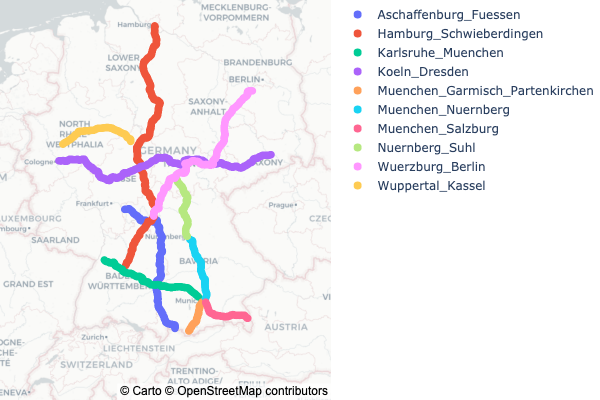
\includegraphics{final_report_files/images/overall_map.png}

}

\caption{Overall\_map}

\end{figure}



\end{document}
